\section{Realisering og test}
\label{sec:research}

Punktprøvingsfrekvensen $f_s$ er satt til 6,4 kHz. Dermed blir spesifikasjonene som plottet i tabell \ref{tab:spec}. 

\begin{table}[ht]
    \caption{Filterspesifikasjoner}
    \centering
    \begin{tabular}{|l|l|l|}
        \hline
        Spesifikasjon & Formel                              & Verdi        \\ \hline
        $f_s$         &                                     & 6400Hz       \\ \hline
        B             & $\frac{f_s}{2}$                     & 3200Hz       \\ \hline
        $f_c$         & $\geq\frac{3}{8}f_s$                & $\geq$2400Hz \\ \hline
    \end{tabular}
    \label{tab:spec}
\end{table}

Ved å ta i bruk formlene gitt i seksjon \ref{sec:concept} blir beregninene som vist i tabell

\begin{table}[hbt]
    \centering
    \caption{Beregninger.}
    % \setlength\extrarowheight{9pt}
    \begin{Large}
    \begin{tabular}{|l|l|l|}
        \hline
        Størrelse   & Formel                                              & Måltall og enhet          \\ \hline
        A           & $10^{\frac{A[dB]}{20}}$                             & $\approx0.3162$           \\ \hline
        n           & $\frac{1}{2}\frac{ln(A^{-2}-1)}{ln(\frac{f}{f_c})}$ & $\approx3.81\rightarrow4$ \\ \hline
        R           &                                                     & $1k\Omega$                \\ \hline
        $\zeta_1$   & tatt fra tabel \ref{tab:polpar}                     & 0.92388                   \\ \hline
        $\zeta_2$   & tatt fra tabel \ref{tab:polpar}                     & 0.38268                   \\ \hline
        $\omega_0$  & $2\pi f_c$                                          & $15079.64\frac{rad}{s}$   \\ \hline
        $\tau_{11}$ & $\frac{1}{\omega_0 \zeta_1}$                        & $71.77\mu s$              \\ \hline
        $\tau_{12}$ & $\frac{1}{\omega_0^2 \tau_{11}}$                    & $61.27\mu s$              \\ \hline
        $\tau_{21}$ & $\frac{1}{\omega_0 \zeta_2}$                        & $173.29\mu s$             \\ \hline
        $\tau_{22}$ & $\frac{1}{\omega_0^2 \tau_{21}}$                    & $25.38\mu s$              \\ \hline
        $C_{11}$      & $\frac{\tau_{11}}{R}$                               & $71.77nf$              \\ \hline
        $C_{12}$      & $\frac{\tau_{12}}{R}$                               & $61.27nf$              \\ \hline
        $C_{21}$      & $\frac{\tau_{21}}{R}$                               & $173.29nf$             \\ \hline
        $C_{22}$      & $\frac{\tau_{22}}{R}$                               & $25.38nf$              \\ \hline
        \end{tabular}
    \end{Large}
    \label{tab:calculations}
    \end{table}

Den realiserte er illustrert i figur \ref{fig:01realised}. Merk at verdiene ikke er det samme som på tabell \ref{tab:calculations} da det er små avvik i kondensatorene, men til tross for det så er avviket relativt lavt.

\begin{figure}[!hbt]
	\centering
	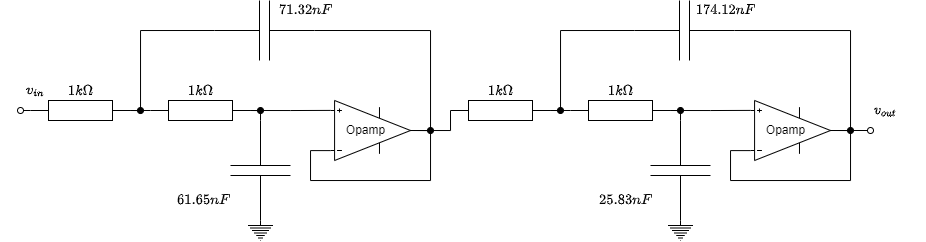
\includegraphics[scale=0.45]{./Images/03Research/01realisertkrets.png}
	\caption{Realisert krets med verdier.}
	\label{fig:01realised}
\end{figure}